\documentclass[a4paper]{article}
\usepackage[top=2cm, bottom=2cm, outer=0cm, inner=0cm]{geometry}
\usepackage[pages=some]{background}
\usepackage{graphicx}
\usepackage[absolute,overlay]{textpos}
%\usepackage{fontspec}
\usepackage{setspace}
\usepackage{ifthen}
\usepackage{hyperref}

\newboolean{IsAufenthaltstitel}
\newboolean{IsVorabzustimmung}
\newboolean{IsErsterteilung}
\newboolean{IsVerlaengerung}

\newboolean{IsWeiblich}
\newboolean{IsMaennlich}
\newboolean{IsDivers}

\newboolean{IsNeueinreise}
\newboolean{IsVerlaengerungI}
\newboolean{IsBefristet}

\newboolean{IsLeiharbeiter}

\newboolean{IsArbeitsort}

\newboolean{IsKein Abschluss}
\newboolean{IsHochschule}
\newboolean{IsBerufsausbildung}
\newboolean{IsSonstige Ausbildung}
\newboolean{IsAbschlussVergleichbar}
\newboolean{IsBeruflicheAnerkennungJa}
\newboolean{IsBeruflicheAnerkennungNein}
\newboolean{IsBeruflicheAnerkennungTeilweise}
\newboolean{IsSonstigeAusbildung}
\newboolean{IsKeineAusbildungFreiwillig}

\newboolean{IsBerufsausuebungserlaubnis}

\newboolean{IsUeberstundenpflicht}

\newboolean{IsVollzeit}
\newboolean{IsTeilzeit}
\newboolean{IsGeringfuegigeBeschaeftigung}

\newboolean{IsTarifvertrag}
\newboolean{IsVereinbarungArbeitsvertrag}
\newboolean{IsLohn}
\newboolean{IsGehalt}

\newboolean{IsProStunde}
\newboolean{IsProMonat}
\newboolean{IsGeldwerteLeistung}
\newboolean{IsSonstigeBerechnung}

\newboolean{IsSozialversicherungspflicht}

\newboolean{IsRueckstaendeSozSteu}
\newboolean{IsStrafBussgeld}
\newboolean{IsInsolvenz}
\newboolean{IsInsolvenzAbgelehnt}
\newboolean{IsVerwandtschaft}



% Info page one
\setboolean{IsAufenthaltstitel}{false}
\setboolean{IsVorabzustimmung}{true}
\setboolean{IsErsterteilung}{false}
\setboolean{IsVerlaengerung}{true}

\newcommand{\Name}{Mustermann}
\newcommand{\Vorname}{Max}
\setboolean{IsWeiblich}{true}
\setboolean{IsMaennlich}{false}
\setboolean{IsDivers}{false}

\newcommand{\Geburtsdatum}{01.02.1994}
\newcommand{\Staatsangehörigkeit}{mexikanisch}
\newcommand{\Aufenthaltsort}{Manila}

\newcommand{\Firma}{Social-Bee gGmbH}
\newcommand{\Kontaktperson}{Sasheen Teisner}
\newcommand{\TelefonNummer}{089/18914481}
\newcommand{\Straße}{St.-Martin-Straße 112}
\newcommand{\PLZOrt}{81669 München}
\newcommand{\Fax}{089/24887906}
\newcommand{\EMail}{sasheen.teisner@social-bee.de}
\newcommand{\Betriebsnummer}{95695562}

\setboolean{IsNeueinreise}{true}
\newcommand{\beginnt}{}
\setboolean{IsVerlaengerungI}{false}
\newcommand{\besteht}{}
\setboolean{IsBefristet}{true}
\newcommand{\befristet}{}

\setboolean{IsLeiharbeiter}{true}

\setboolean{IsArbeitsort}{true}
\newcommand{\Ort}{Raum München}

% Info page two
\newcommand{\BeschreibungTaetigkeit}{Helfertätigkeiten in Stellen der Produktionsbranche, in Lager und Logistik, im Verkauf, bei Verwaltungsaufgaben und Bürotätigkeiten, in der Gastronomie, im Hotelgewerbe, im Baunebengewerbe, im Pflegebereich.}

\setboolean{IsKein Abschluss}{true}
\setboolean{IsHochschule}{false}
\newcommand{\AbschlussArt}{}
\newcommand{\AbschlussOrt}{}
\setboolean{IsAbschlussVergleichbar}{false}
\newcommand{\NachweisAbschluss}{}
\setboolean{IsBerufsausbildung}{false}
\newcommand{\Berufsausbildung}{}
\newcommand{\BerufsausbildungOrt}{}
\setboolean{IsBeruflicheAnerkennungJa}{false}
\setboolean{IsBeruflicheAnerkennungNein}{false}
\setboolean{IsBeruflicheAnerkennungTeilweise}{false}
\newcommand{\Nachweis}{}
\setboolean{IsSonstigeAusbildung}{true}
\newcommand{\Faehigkeiten}{Deutschkenntnisse A2}
\setboolean{IsKeineAusbildungFreiwillig}{true}
\newcommand{\FreiwilligeAngabe}{}


% Info page three
\setboolean{IsBerufsausuebungserlaubnis}{false}
\newcommand{\QualifikationErlaubnis}{}

\setboolean{IsVollzeit}{true}
\newcommand{\Vollzeit}{35}
\setboolean{IsTeilzeit}{false}
\newcommand{\Teilzeit}{}
\setboolean{IsGeringfuegigeBeschaeftigung}{false}
\newcommand{\GeringfuegigeBeschaeftigung}{}

\setboolean{IsUeberstundenpflicht}{false}
\newcommand{\Ueberstundenzahl}{}
\newcommand{\Ueberstundenausgleich}{}

\newcommand{\ArbeitstageProUrlaubsjahr}{24}


\setboolean{IsTarifvertrag}{true}
\newcommand{\Tarifvertrag}{IGZ}
\newcommand{\Entgeltgruppe}{1}
\setboolean{IsVereinbarungArbeitsvertrag}{false}
\setboolean{IsLohn}{true}
\setboolean{IsGehalt}{false}

\setboolean{IsProStunde}{true}
\newcommand{\Stunde}{10,45 Euro}
\setboolean{IsProMonat}{false}
\newcommand{\ProMonat}{}
\setboolean{IsGeldwerteLeistung}{false}
\newcommand{\GeldwerteLeistungForm}{}
\newcommand{\GeldwerteLeistung}{}
\setboolean{IsSonstigeBerechnung}{false}
\newcommand{\SonstigeBerechnung}{}

\setboolean{IsSozialversicherungspflicht}{true}
\newcommand{\KeineSozialversicherungspflicht}{}

\setboolean{IsRueckstaendeSozSteu}{false}
\setboolean{IsStrafBussgeld}{false}
\setboolean{IsInsolvenz}{false}
\setboolean{IsInsolvenzAbgelehnt}{false}
\newcommand{\Gruendungsjahr}{2016}
\newcommand{\AnzahlAN}{124}
\setboolean{IsVerwandtschaft}{false}
\newcommand{\Amtsgericht}{}
\newcommand{\Registernummer}{}
\newcommand{\WeitereAngabenSvier}{}

\newcommand{\OrtDatum}{Hamburg, \today}









\backgroundsetup{
scale=1,
color=black,
opacity=1,
angle=0,
contents={%
  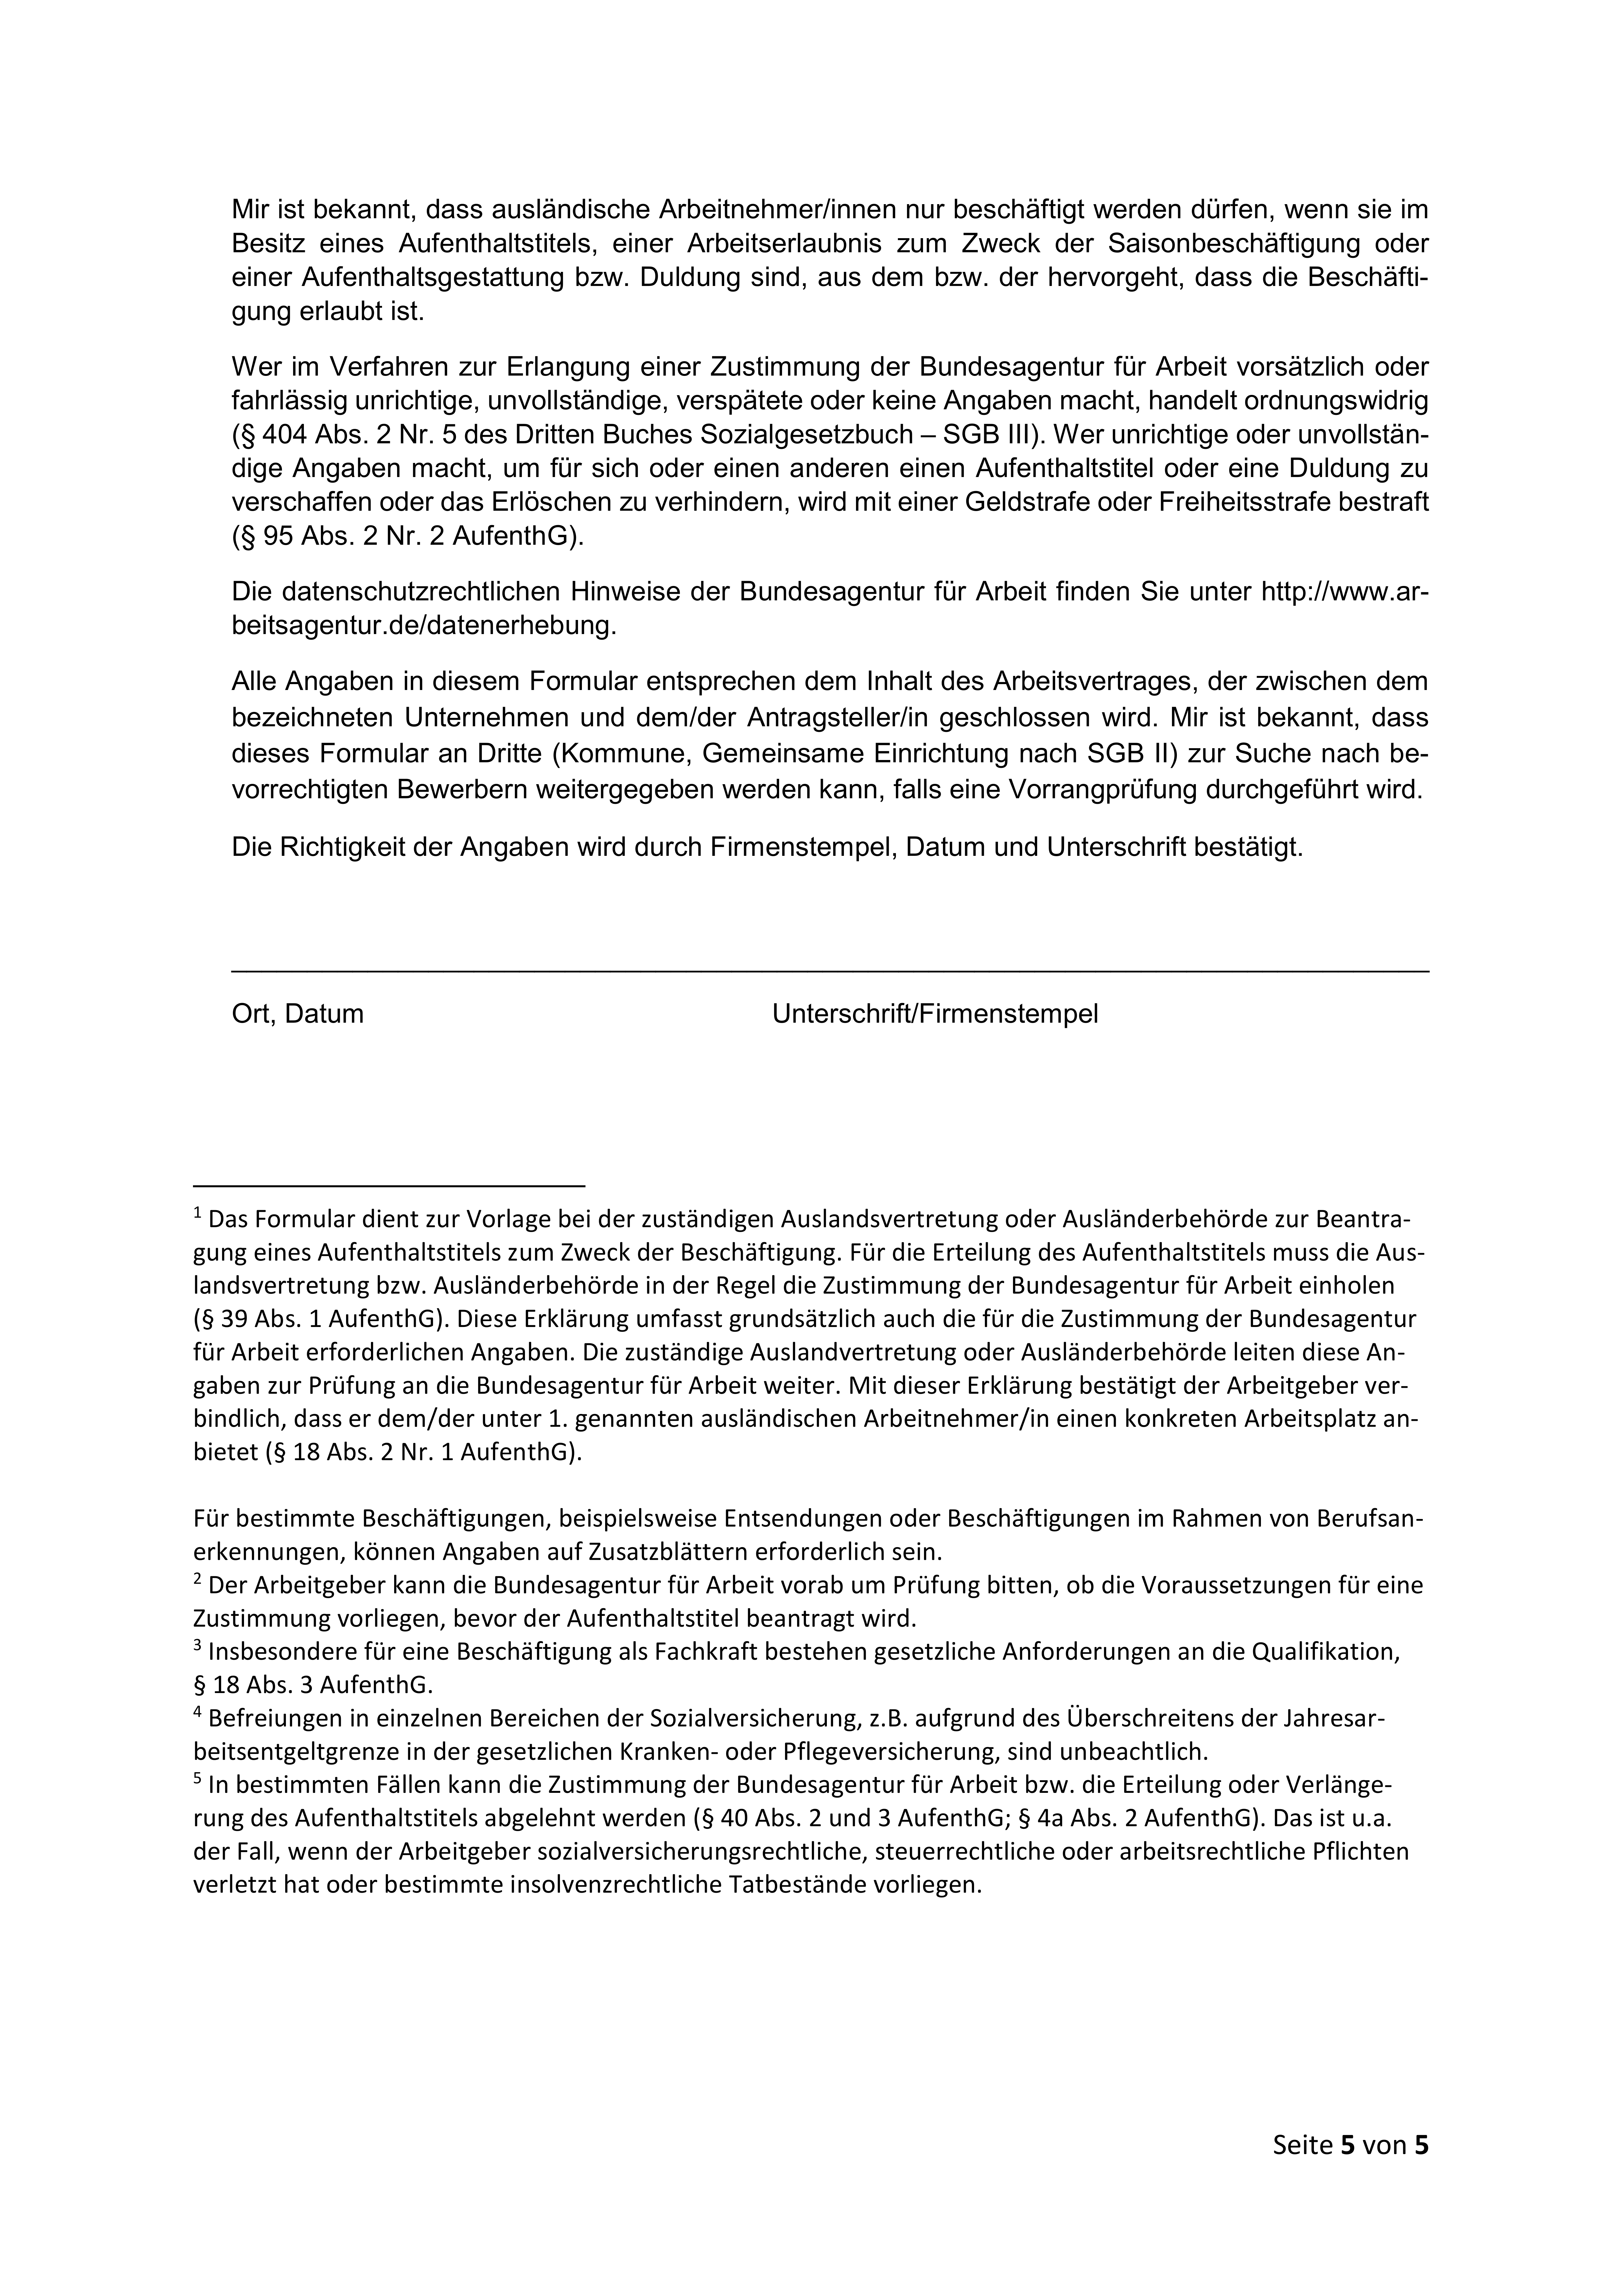
\includegraphics[width=\paperwidth,height=\paperheight]{s5_Erklaerung_zum_Beschaeftigungsverhaeltnis-000005}
  }%
}

\begin{document}
\begin{Form}

\backgroundsetup{
  scale=1,
  color=black,
  opacity=1,
  angle=0,
  contents={%
    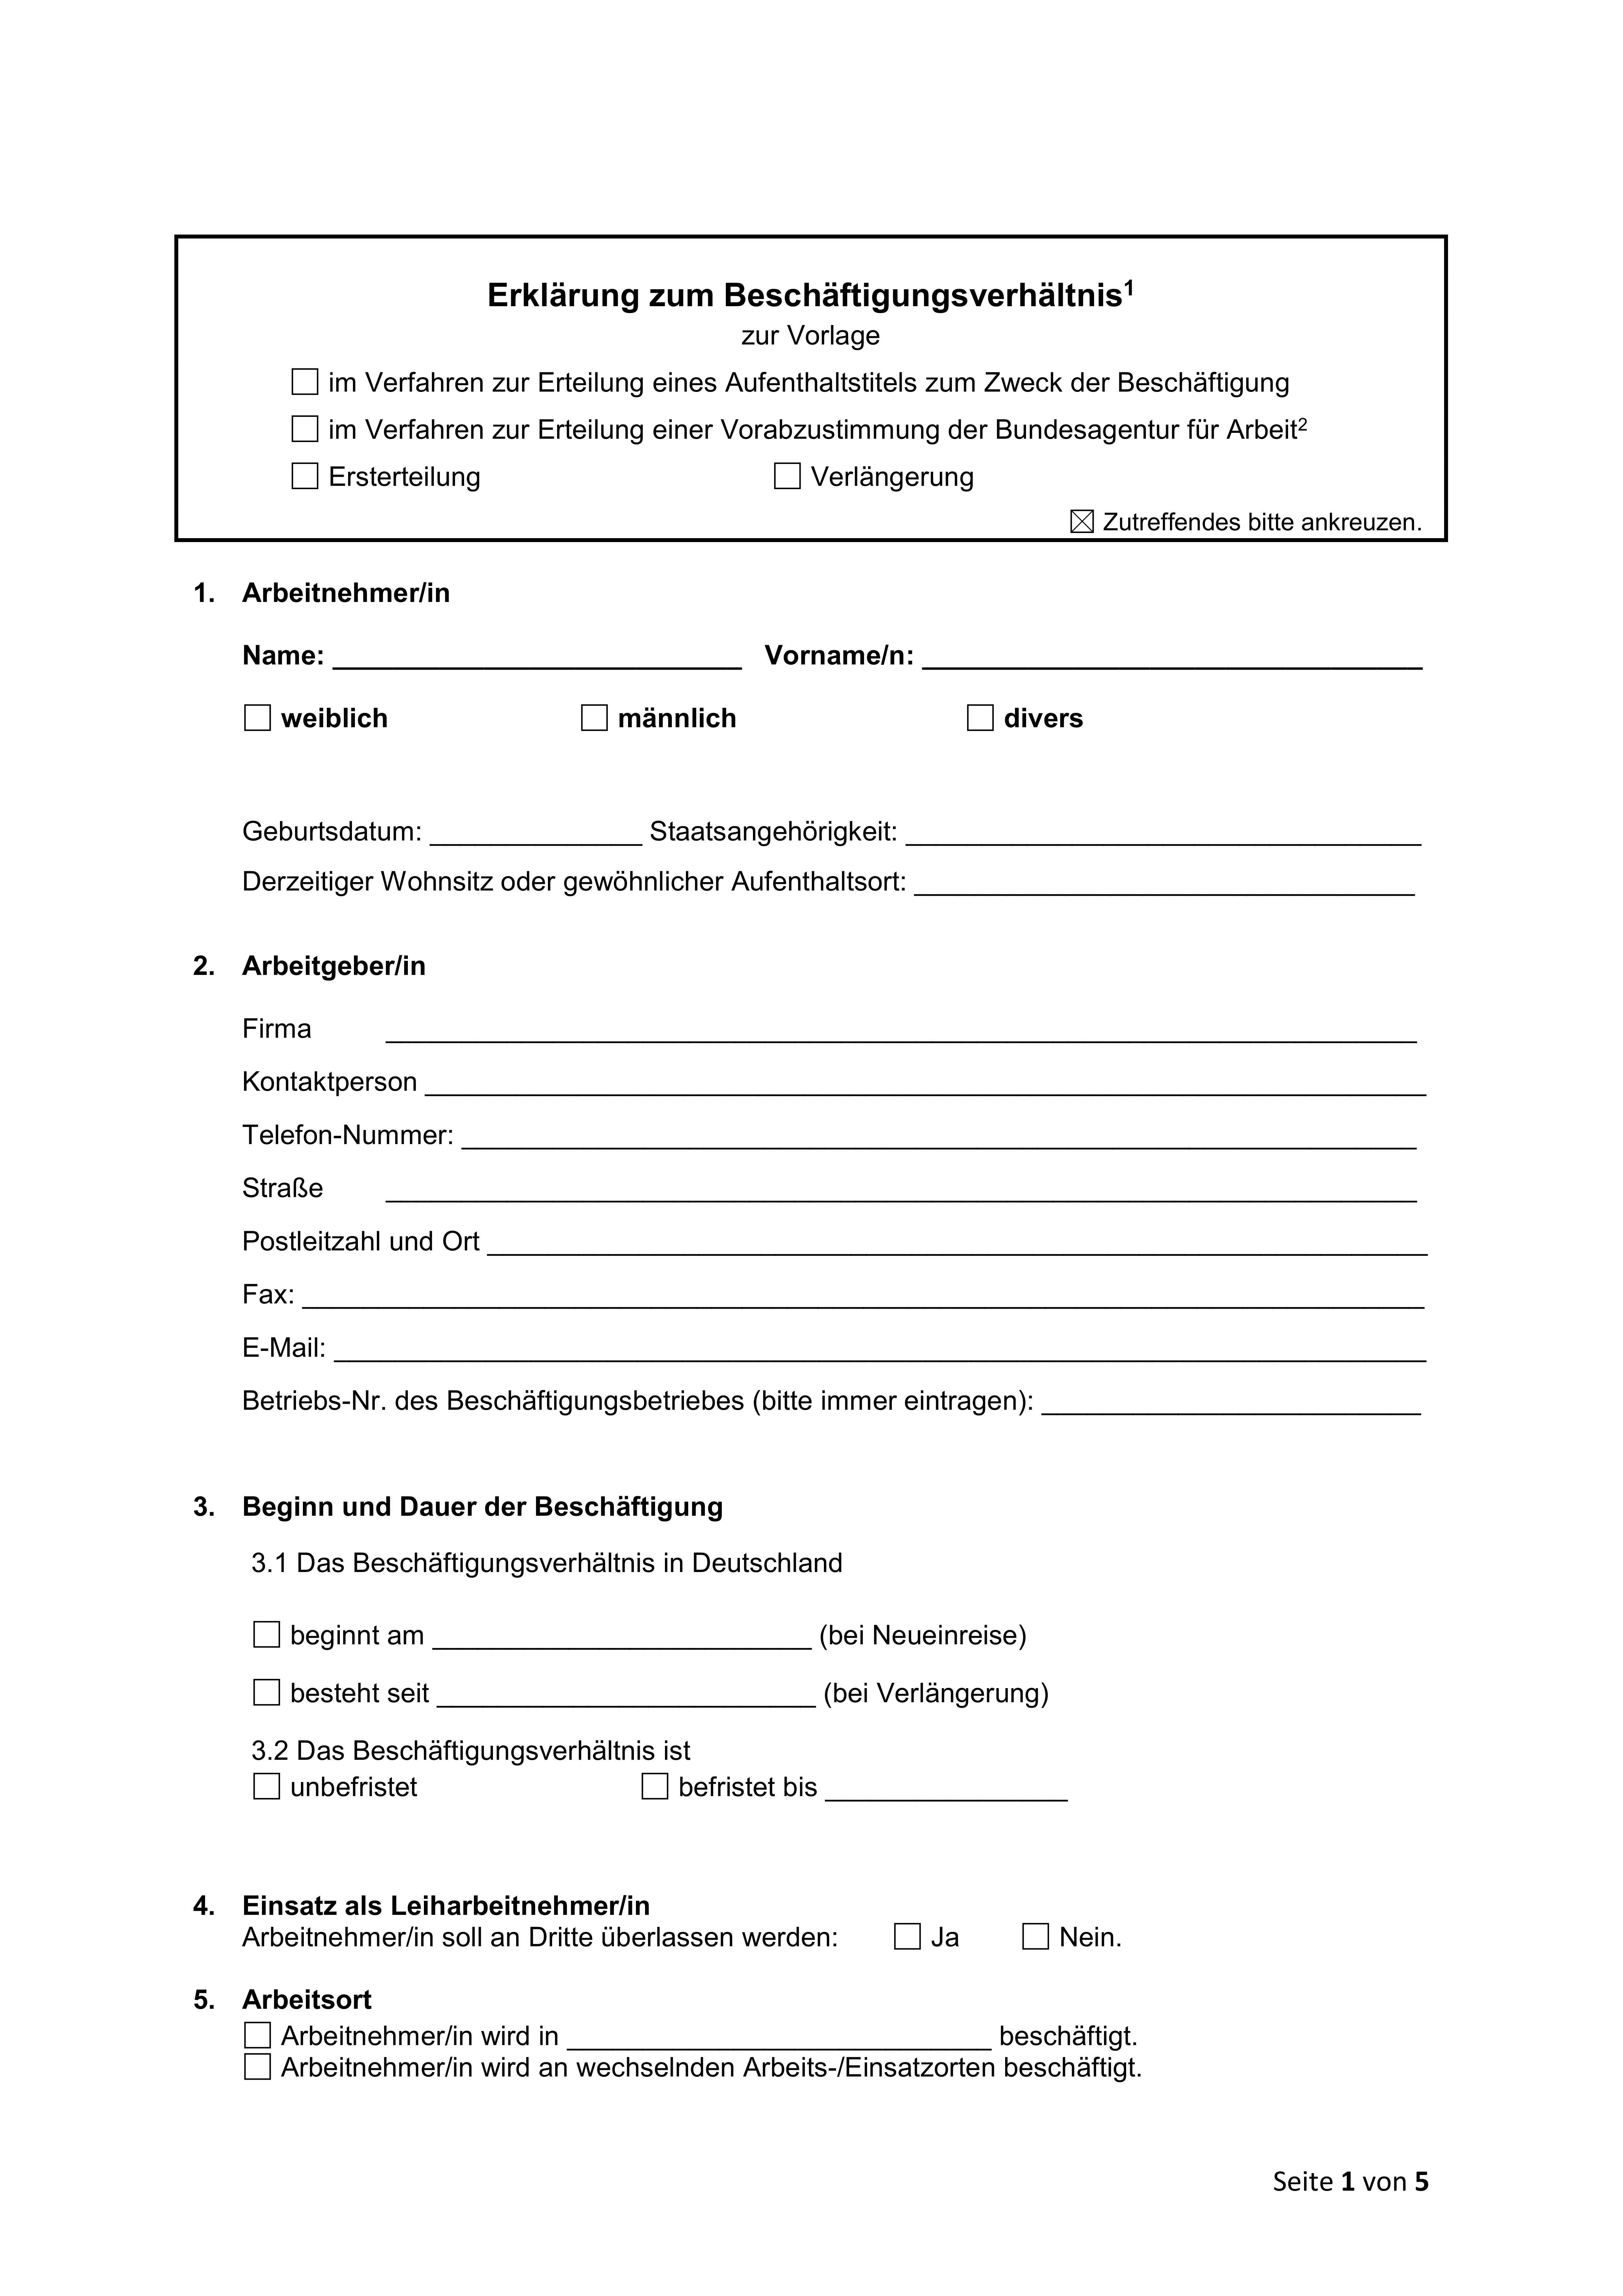
\includegraphics[width=\paperwidth,height=\paperheight]{s1_Erklaerung_zum_Beschaeftigungsverhaeltnis-000001}
    }%
}
\BgThispage

\begin{textblock*}{0.3cm}(3.25cm,4.78cm) % {block width} (coords) 
  %\ifthenelse{\boolean{IsAufenthaltstitel}}{x}{}
  \CheckBox[name=aufenthaltstitelCheck, checked=IsAufenthaltstitel, height=0.3cm, width=0.3cm, checkboxsymbol=\ding{53}]{}
\end{textblock*}

\begin{textblock*}{0.3cm}(3.25cm,5.4cm) % {block width} (coords) 
  \CheckBox[name=vorabzustimmungCheck, checked=IsVorabzustimmung, height=0.3cm, width=0.3cm, checkboxsymbol=\ding{53}]{}
\end{textblock*}

\begin{textblock*}{0.3cm}(3.35cm,6.1cm) % {block width} (coords) 
\ifthenelse{\boolean{IsErsterteilung}}{x}{}
\end{textblock*}

\begin{textblock*}{0.3cm}(9.6cm,6.1cm) % {block width} (coords) 
\ifthenelse{\boolean{IsVerlaengerung}}{x}{}
\end{textblock*}


%Arbeitnehmer/in
\begin{textblock*}{5.3cm}(3.8cm,8.25cm) % {block width} (coords) 
  %\Name
  \TextField[name=nameTextField, backgroundcolor=gray!20, borderwidth=0, width=5.3cm, value={\Name}]{}
\end{textblock*}

\begin{textblock*}{6.5cm}(11.5cm,8.35cm) % {block width} (coords) 
  \Vorname
\end{textblock*}

\begin{textblock*}{0.3cm}(2.722cm,9.23cm) % {block width} (coords) 
  \ifthenelse{\boolean{IsWeiblich}}{x}{}
\end{textblock*}

\begin{textblock*}{0.3cm}(7.08cm,9.23cm) % {block width} (coords) 
  \ifthenelse{\boolean{IsMaennlich}}{x}{}
\end{textblock*}

\begin{textblock*}{0.3cm}(12.059cm,9.23cm) % {block width} (coords) 
  \ifthenelse{\boolean{IsDivers}}{x}{}
\end{textblock*}

\begin{textblock*}{2.8cm}(5.1cm,10.65cm) % {block width} (coords) 
 \Geburtsdatum
\end{textblock*}

\begin{textblock*}{6.7cm}(11.3cm,10.64cm) % {block width} (coords) 
\Staatsangehörigkeit
\end{textblock*}

\begin{textblock*}{6cm}(11.4cm,11.28cm) % {block width} (coords) 
\Aufenthaltsort
\end{textblock*}

%Arbeitgeber/in
\begin{textblock*}{13,4cm}(4.5cm,13.2cm) % {block width} (coords) 
\Firma
\end{textblock*}

\begin{textblock*}{13cm}(5cm,13.87cm) % {block width} (coords) 
\Kontaktperson
\end{textblock*}

\begin{textblock*}{12.4cm}(5.48cm,14.57cm) % {block width} (coords) 
\TelefonNummer
\end{textblock*}

\begin{textblock*}{13.4cm}(4.49cm,15.26cm) % {block width} (coords) 
\Straße
\end{textblock*}

\begin{textblock*}{12.2cm}(5.78cm,15.95cm) % {block width} (coords) 
\PLZOrt
\end{textblock*}

\begin{textblock*}{14.6cm}(3.47cm,16.65cm) % {block width} (coords) 
\Fax
\end{textblock*}

\begin{textblock*}{14.2cm}(3.8cm,17.32cm) % {block width} (coords) 
\EMail
\end{textblock*}

\begin{textblock*}{5cm}(13cm,18.04cm) % {block width} (coords) 
\Betriebsnummer
\end{textblock*}

%Beginn und Dauer der Beschäftigung
%3.1
\begin{textblock*}{0.3cm}(2.84cm,21.06cm) % {block width} (coords) 
 \ifthenelse{\boolean{IsNeueinreise}}{x}{}
\end{textblock*}

\begin{textblock*}{5cm}(5.19cm,21.08cm) % {block width} (coords) 
\beginnt
\end{textblock*}

\begin{textblock*}{0.3cm}(2.84cm,21.85cm) % {block width} (coords) 
 \ifthenelse{\boolean{IsVerlaengerungI}}{x}{}
\end{textblock*}

\begin{textblock*}{5cm}(5.19cm,21.82cm) % {block width} (coords) 
\besteht
\end{textblock*}

%3.2
\begin{textblock*}{0.3cm}(2.84cm,23.06cm) % {block width} (coords) 
 \ifthenelse{\boolean{IsBefristet}}{}{x}
\end{textblock*}

\begin{textblock*}{0.3cm}(7.87cm,23.06cm) % {block width} (coords) 
 \ifthenelse{\boolean{IsBefristet}}{x}{}
\end{textblock*}

\begin{textblock*}{3.2cm}(10.23cm,23.03cm) % {block width} (coords) 
 \ifthenelse{\boolean{IsBefristet}}{\befristet}{}
\end{textblock*}

%Einsatz als Leiharbeitnehmer/in
\begin{textblock*}{0.3cm}(11.13cm,25cm) % {block width} (coords) 
 \ifthenelse{\boolean{IsLeiharbeiter}}{x}{}
\end{textblock*}

\begin{textblock*}{0.3cm}(12.8cm,25cm) % {block width} (coords) 
 \ifthenelse{\boolean{IsLeiharbeiter}}{}{x}
\end{textblock*}

%Arbeitsort
\begin{textblock*}{0.3cm}(2.74cm,26.25cm) % {block width} (coords) 
 \ifthenelse{\boolean{IsArbeitsort}}{x}{}
\end{textblock*}

\begin{textblock*}{5.55cm}(6.85cm,26.24cm) % {block width} (coords) 
 \ifthenelse{\boolean{IsArbeitsort}}{\Ort}{}
\end{textblock*}

\begin{textblock*}{0.3cm}(2.74cm,26.67cm) % {block width} (coords) 
  \ifthenelse{\boolean{IsArbeitsort}}{}{x}
\end{textblock*}

~\clearpage


\backgroundsetup{
scale=1,
color=black,
opacity=0.8,
angle=0,
contents={%
  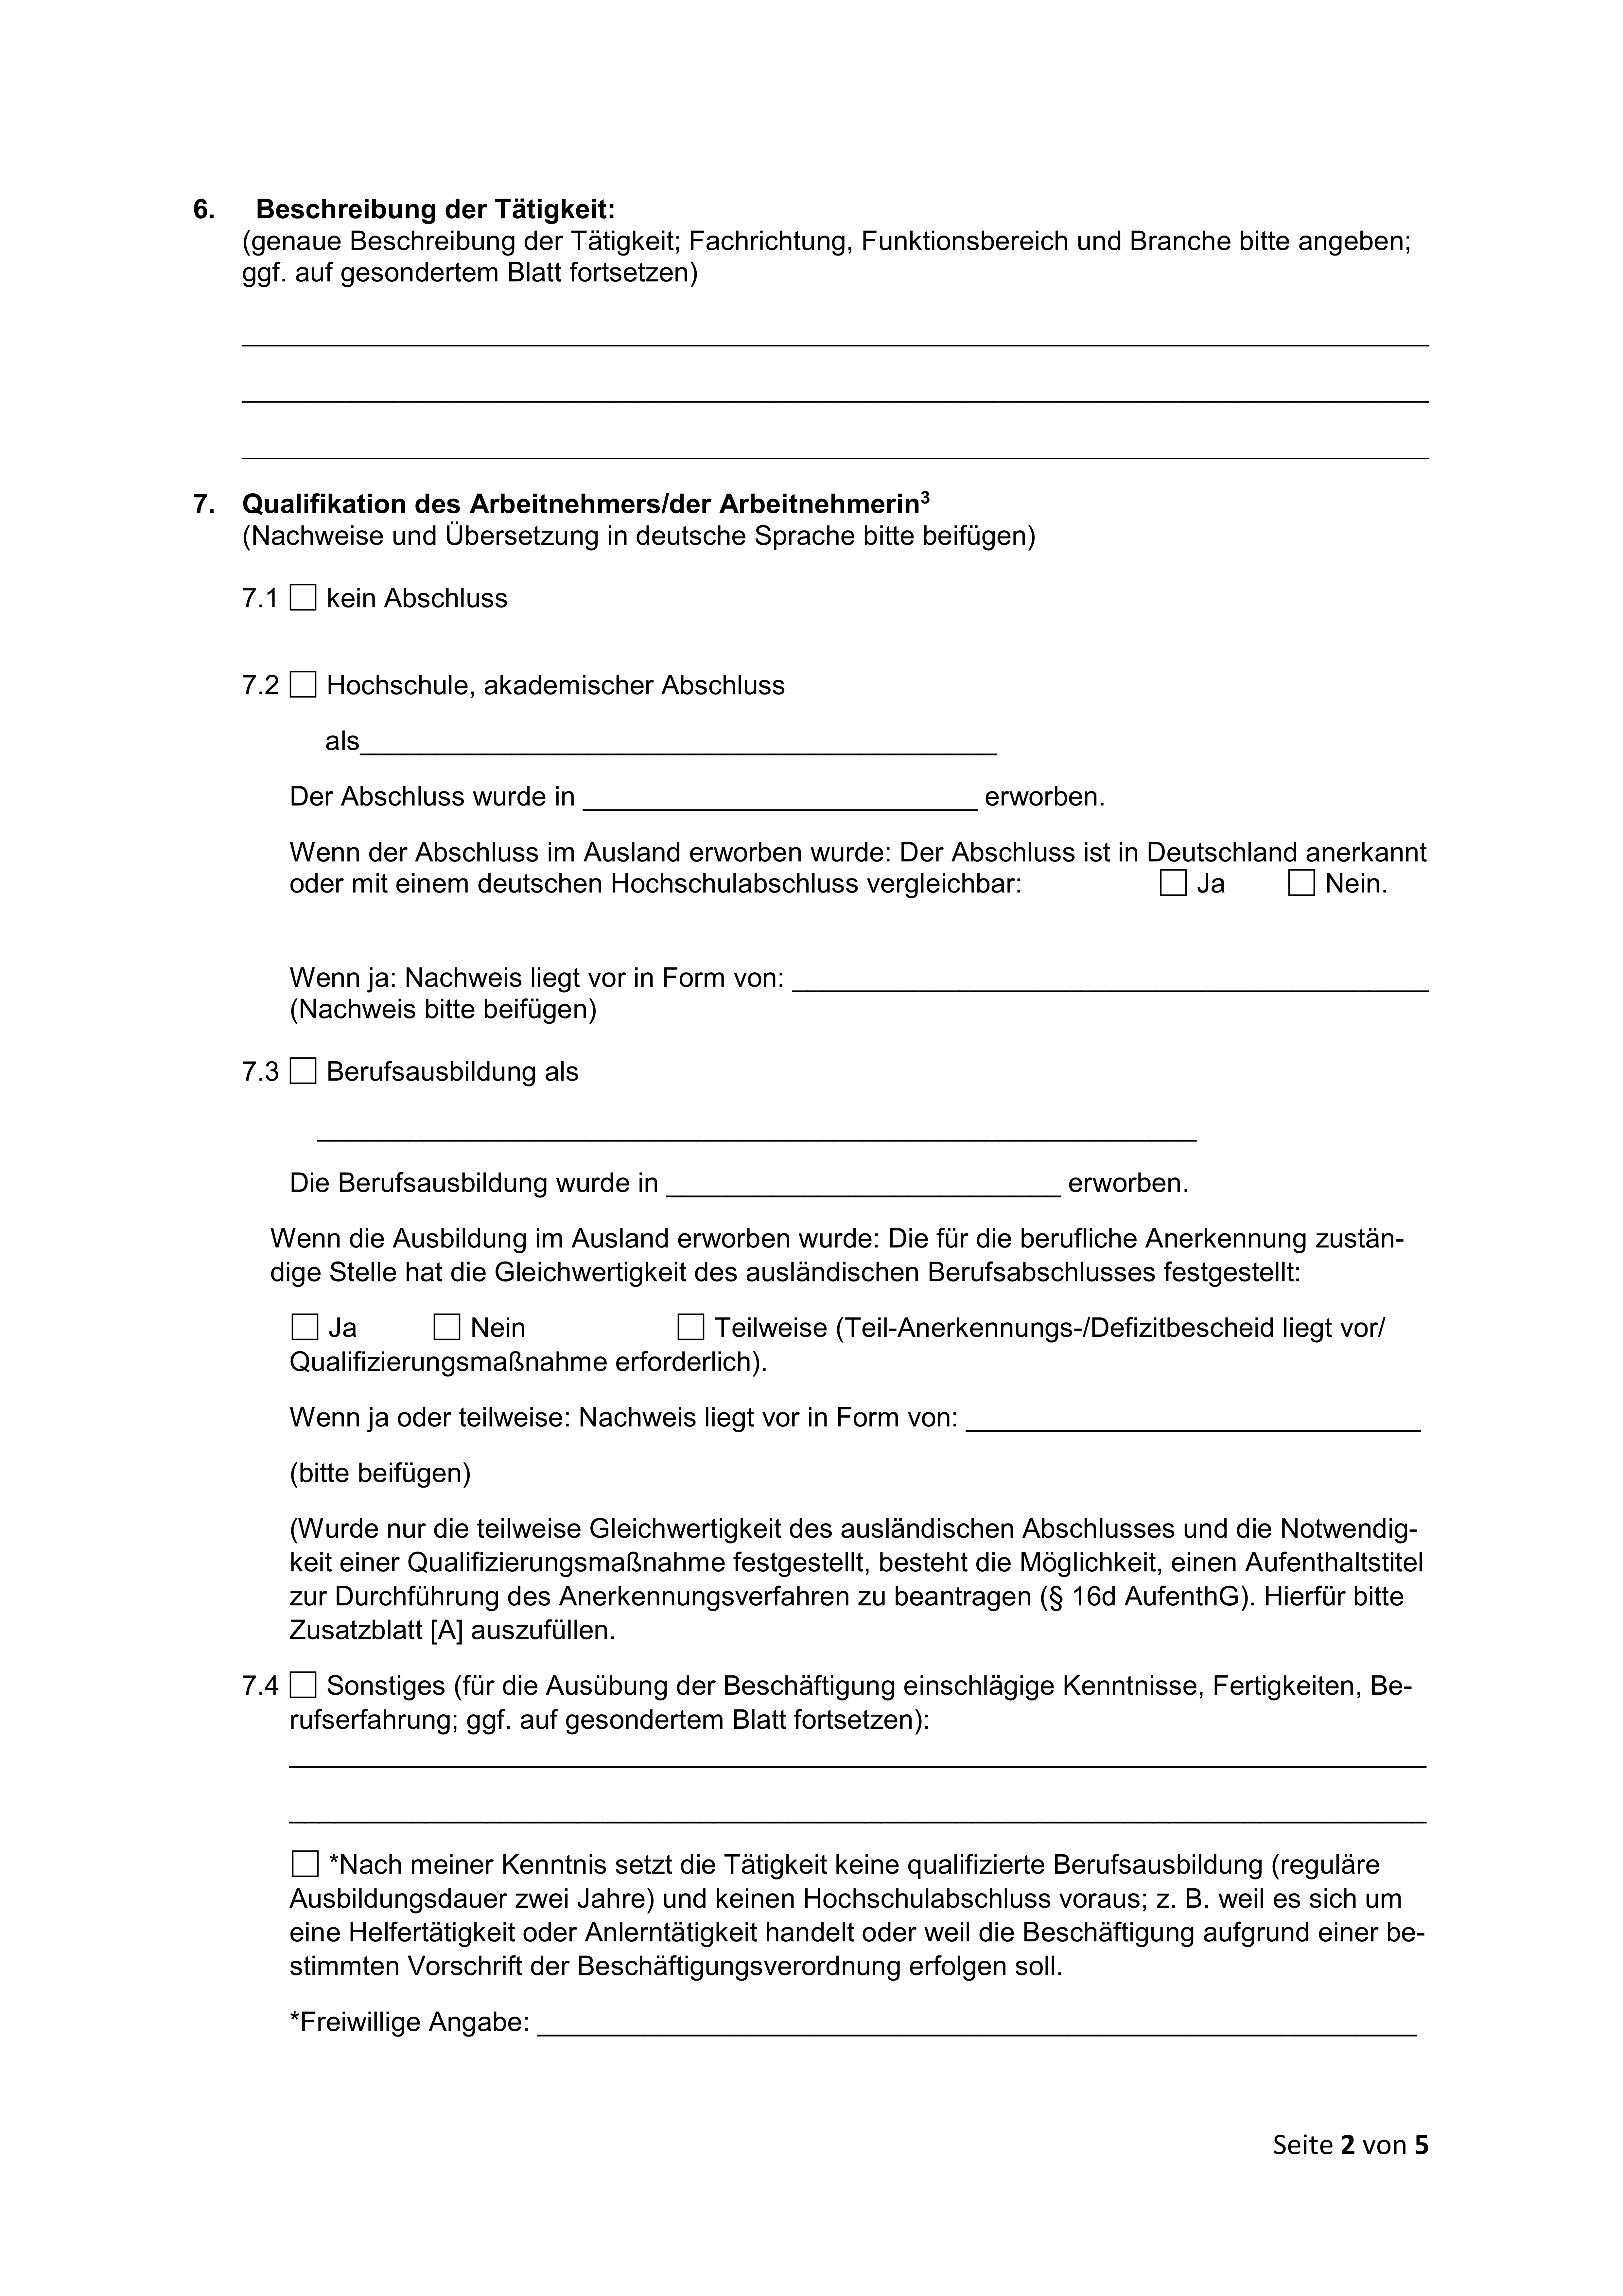
\includegraphics[width=\paperwidth,height=\paperheight]{s2_Erklaerung_zum_Beschaeftigungsverhaeltnis-000002}
  }%
}


 \BgThispage
%Beschreibung der Tätigkeit
\begin{textblock*}{15.4cm\setstretch{1.75}}(3.2cm,4.2cm) % {block width} (coords)
\noindent
\BeschreibungTaetigkeit
\end{textblock*}

%Qualifikation des Arbeitnehmers
%7.1
\begin{textblock*}{0.3cm}(3.3cm,7.66cm) % {block width} (coords) 
 \ifthenelse{\boolean{IsKein Abschluss}}{x}{}
\end{textblock*}

%7.2
\begin{textblock*}{0.3cm}(3.3cm,8.77cm) % {block width} (coords) 
 \ifthenelse{\boolean{IsHochschule}}{x}{}
\end{textblock*}

\begin{textblock*}{8.3cm\setstretch{1.75}}(4.69cm,9.48cm) % {block width} (coords)
\noindent
\AbschlussArt
\end{textblock*}

\begin{textblock*}{5.1cm\setstretch{1.75}}(7.6cm,10.22cm) % {block width} (coords)
\noindent
\AbschlussOrt
\end{textblock*}

\begin{textblock*}{0.3cm}(14.58cm,11.35cm) % {block width} (coords) 
 \ifthenelse{\boolean{IsAbschlussVergleichbar}}{x}{}
\end{textblock*}

\begin{textblock*}{0.3cm}(16.242cm,11.35cm) % {block width} (coords) 
 \ifthenelse{\boolean{IsAbschlussVergleichbar}}{}{x}
\end{textblock*}

\begin{textblock*}{8.3cm\setstretch{1.75}}(10.3cm,12.55cm) % {block width} (coords)
\noindent
\NachweisAbschluss
\end{textblock*}

%Berufsausbildung als
\begin{textblock*}{0.3cm}(3.3cm,13.8cm) % {block width} (coords) 
 \ifthenelse{\boolean{IsBerufsausbildung}}{x}{}
\end{textblock*}

\begin{textblock*}{11.4cm\setstretch{1.75}}(4.1cm,14.48cm) % {block width} (coords)
\noindent
\Berufsausbildung
\end{textblock*}

\begin{textblock*}{5.1cm\setstretch{1.75}}(8.68cm,15.2cm) % {block width} (coords)
\noindent
\BerufsausbildungOrt
\end{textblock*}

\begin{textblock*}{0.38cm}(3.33cm,17.1cm) % {block width} (coords) 
 \ifthenelse{\boolean{IsBeruflicheAnerkennungJa}}{x}{}
\end{textblock*}

\begin{textblock*}{0.38cm}(5.18cm,17.1cm) % {block width} (coords) 
 \ifthenelse{\boolean{IsBeruflicheAnerkennungNein}}{x}{}
\end{textblock*}

\begin{textblock*}{0.38cm}(8.33cm,17.1cm) % {block width} (coords) 
 \ifthenelse{\boolean{IsBeruflicheAnerkennungTeilweise}}{x}{}
\end{textblock*}

\begin{textblock*}{5.9cm\setstretch{1.75}}(12.55cm,18.252cm) % {block width} (coords)
\noindent
\Nachweis
\end{textblock*}

\begin{textblock*}{0.38cm}(3.32cm,21.74cm) % {block width} (coords) 
 \ifthenelse{\boolean{IsSonstigeAusbildung}}{x}{}
\end{textblock*}

\begin{textblock*}{15.4cm\setstretch{1.75}}(3.76cm,22.57cm) % {block width} (coords)
\noindent
\Faehigkeiten
\end{textblock*}

\begin{textblock*}{0.38cm}(3.33cm,24.05cm) % {block width} (coords) 
 \ifthenelse{\boolean{IsKeineAusbildungFreiwillig}}{x}{}
\end{textblock*}

\begin{textblock*}{11.4cm\setstretch{1.75}}(7cm,26.05cm) % {block width} (coords)
\noindent
\FreiwilligeAngabe
\end{textblock*}

~\clearpage


\backgroundsetup{
scale=1,
color=black,
opacity=1,
angle=0,
contents={%
  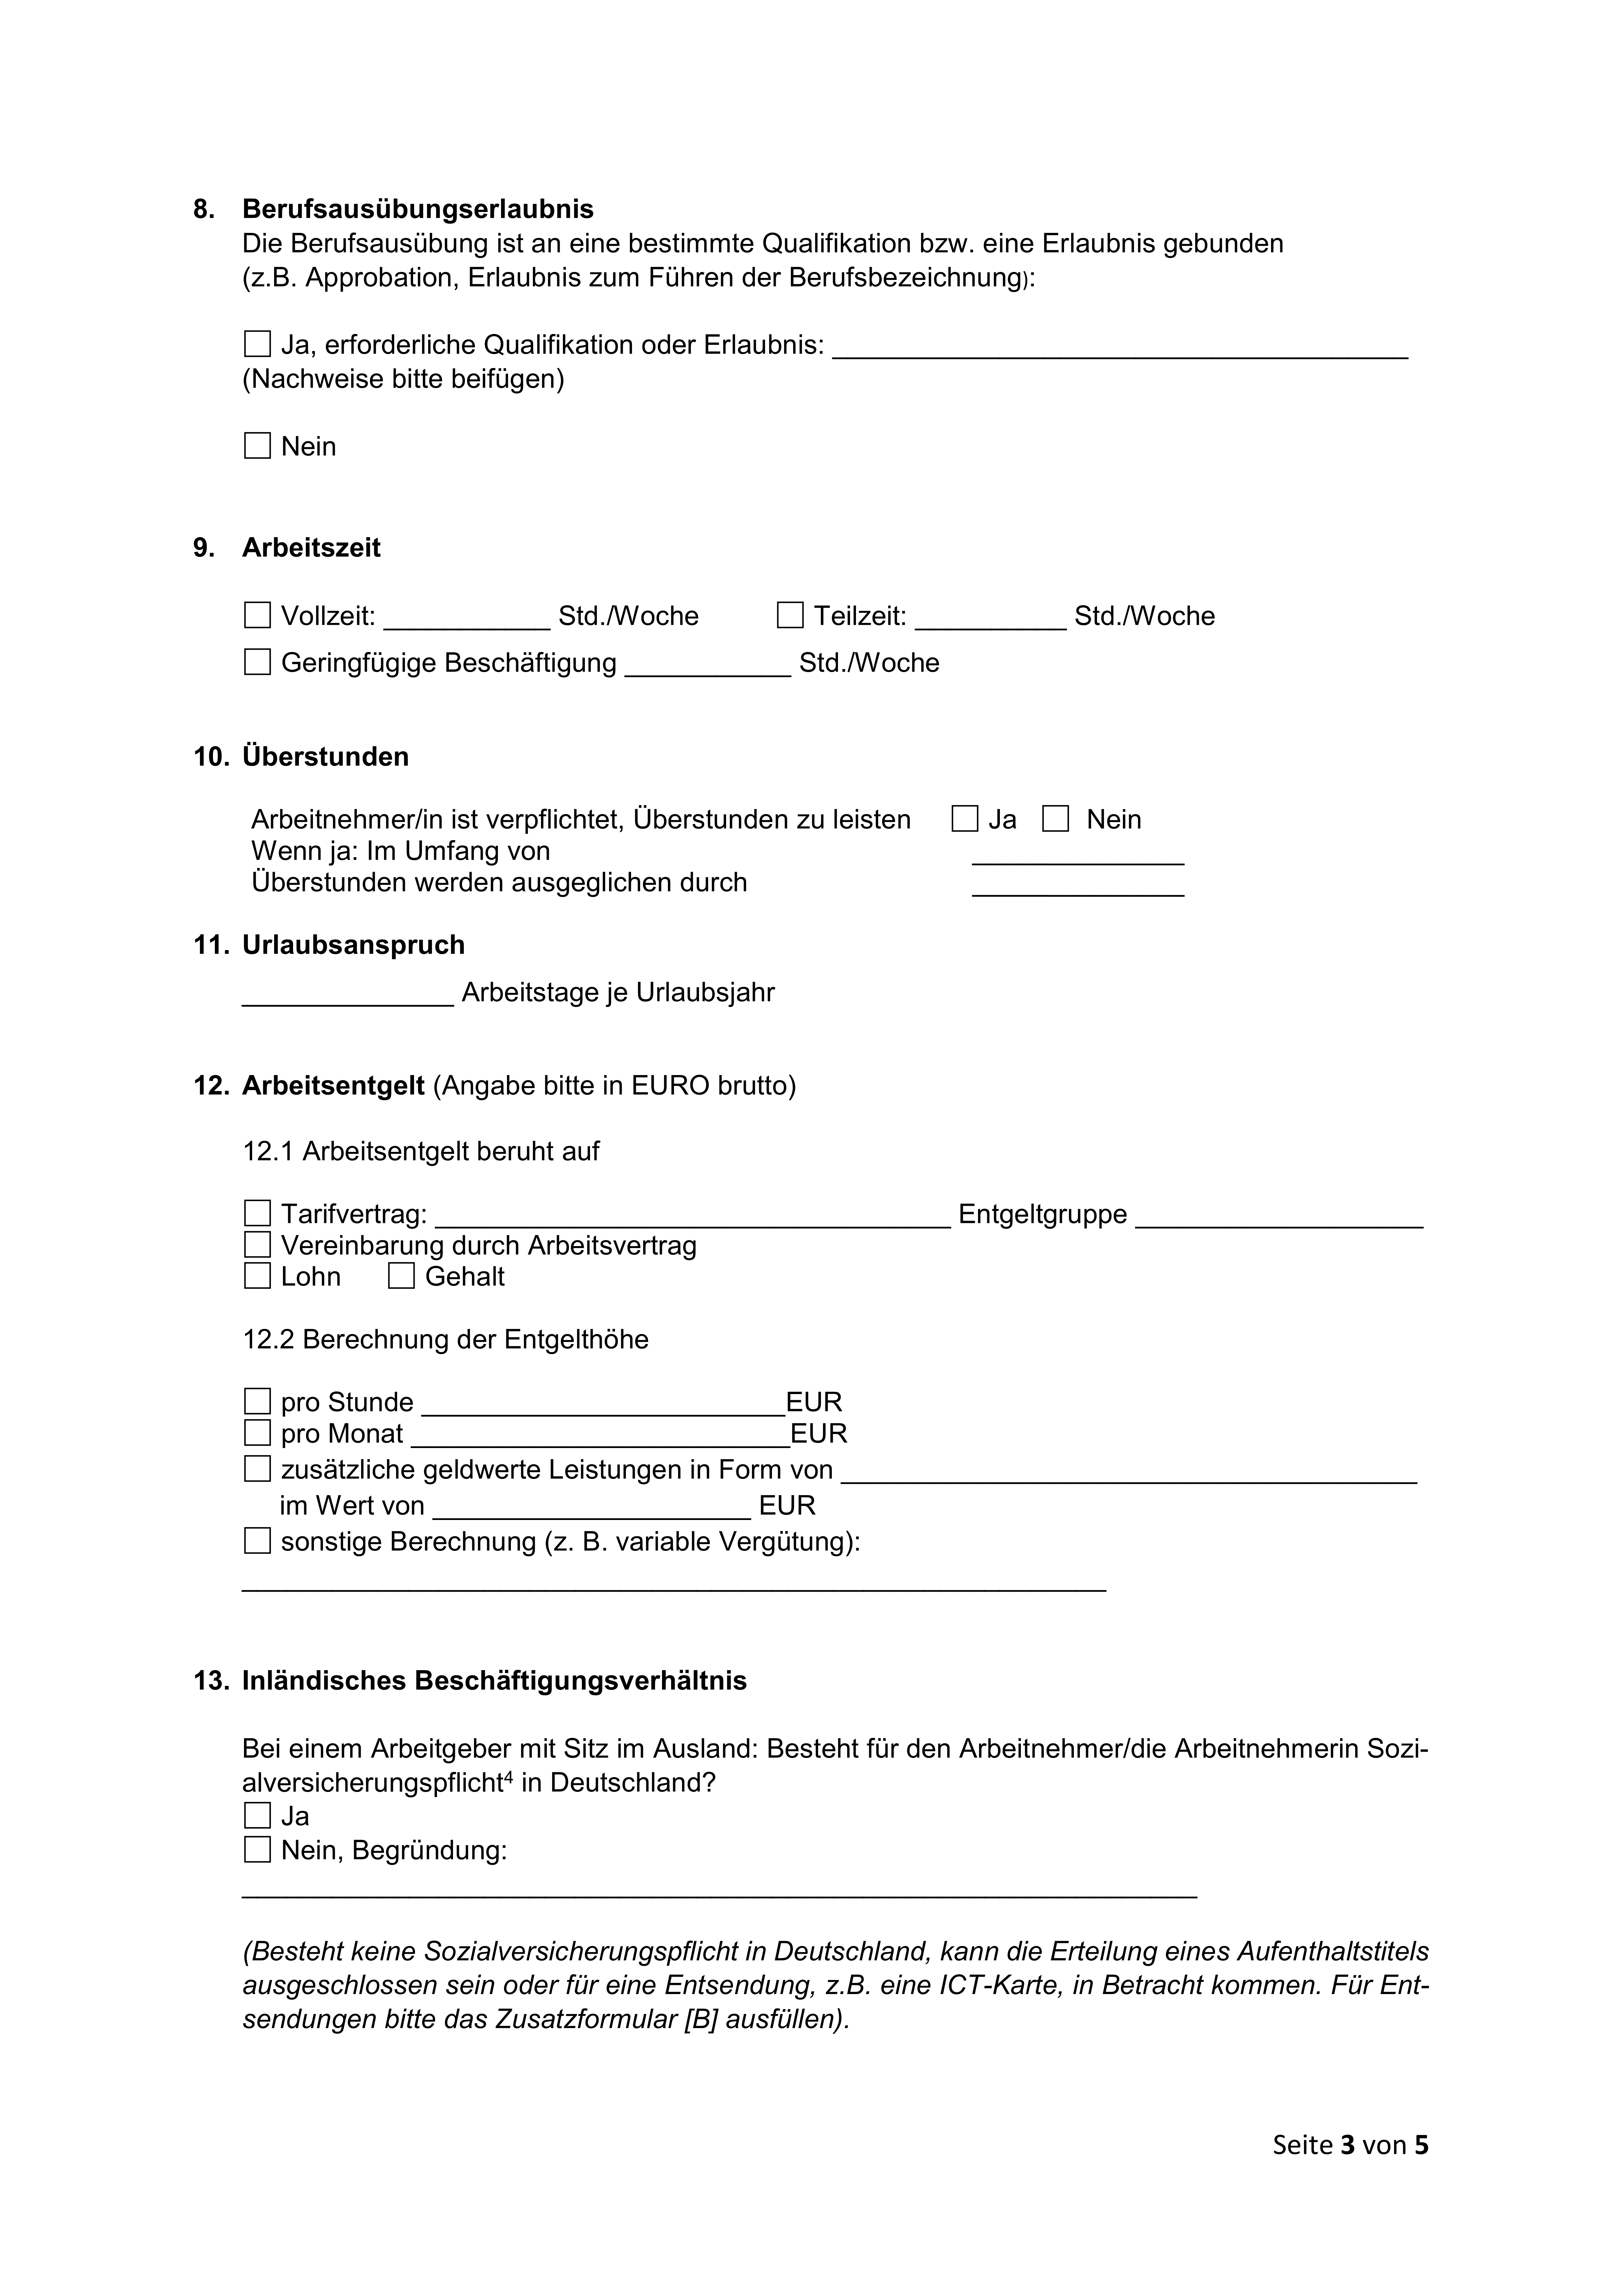
\includegraphics[width=\paperwidth,height=\paperheight]{s3_Erklaerung_zum_Beschaeftigungsverhaeltnis-000003}
  }%
}


 \BgThispage
%Berufsausuebungserlaubnis
\begin{textblock*}{0.3cm\setstretch{1.75}}(3.25cm,4.4cm) % {block width} (coords)
\noindent
 \ifthenelse{\boolean{IsBerufsausuebungserlaubnis}}{x}{}
\end{textblock*}

\begin{textblock*}{7.5cm\setstretch{1.75}}(10.8cm,4.35cm) % {block width} (coords)
\QualifikationErlaubnis
\end{textblock*}

\begin{textblock*}{0.3cm\setstretch{1.75}}(3.25cm,5.7cm) % {block width} (coords)
\noindent
 \ifthenelse{\boolean{IsBerufsausuebungserlaubnis}}{}{x}
\end{textblock*}

%Arbeitszeit
\begin{textblock*}{0.3cm\setstretch{1.75}}(3.25cm,7.9cm) % {block width} (coords)
\noindent
 \ifthenelse{\boolean{IsVollzeit}}{x}{}
\end{textblock*}

\begin{textblock*}{2.2cm\setstretch{1.75}}(5cm,7.87cm) % {block width} (coords)
\noindent
\Vollzeit
\end{textblock*}

\begin{textblock*}{0.3cm\setstretch{1.75}}(10.15cm,7.9cm) % {block width} (coords)
\noindent
 \ifthenelse{\boolean{IsTeilzeit}}{x}{}
\end{textblock*}

\begin{textblock*}{2cm\setstretch{1.75}}(11.9cm,7.9cm) % {block width} (coords)
\noindent
\Teilzeit
\end{textblock*}

\begin{textblock*}{0.3cm\setstretch{1.75}}(3.25cm,8.5cm) % {block width} (coords)
\noindent
 \ifthenelse{\boolean{IsGeringfuegigeBeschaeftigung}}{x}{}
\end{textblock*}

\begin{textblock*}{2cm\setstretch{1.75}}(8.1cm,8.49cm) % {block width} (coords)
\noindent
\GeringfuegigeBeschaeftigung
\end{textblock*}

%Überstunden
\begin{textblock*}{0.3cm\setstretch{1.75}}(12.4cm,10.55cm) % {block width} (coords)
\noindent
 \ifthenelse{\boolean{IsUeberstundenpflicht}}{x}{}
\end{textblock*}

\begin{textblock*}{0.3cm\setstretch{1.75}}(13.57cm,10.55cm) % {block width} (coords)
\noindent
 \ifthenelse{\boolean{IsUeberstundenpflicht}}{}{x}
\end{textblock*}

\begin{textblock*}{2.3cm\setstretch{1.75}}(12.6cm,10.9cm) % {block width} (coords)
\noindent
\Ueberstundenzahl
\end{textblock*}

\begin{textblock*}{2.3cm\setstretch{1.75}}(12.6cm,11.34cm) % {block width} (coords)
\noindent
\Ueberstundenausgleich
\end{textblock*}

%Urlaubsanspruch
\begin{textblock*}{2.3cm\setstretch{1.75}}(3.2cm,12.75cm) % {block width} (coords)
\noindent
\ArbeitstageProUrlaubsjahr
\end{textblock*}

%Arbeitsentgelt
\begin{textblock*}{0.3cm\setstretch{1.75}}(3.25cm,15.63cm) % {block width} (coords)
\noindent
 \ifthenelse{\boolean{IsTarifvertrag}}{x}{}
\end{textblock*}

\begin{textblock*}{6.7cm\setstretch{1.75}}(5.6cm,15.61cm) % {block width} (coords)
\noindent
\Tarifvertrag
\end{textblock*}

\begin{textblock*}{3.7cm\setstretch{1.75}}(14.7cm,15.61cm) % {block width} (coords)
\noindent
\Entgeltgruppe
\end{textblock*}

\begin{textblock*}{0.3cm\setstretch{1.75}}(3.25cm,16.06cm) % {block width} (coords)
\noindent
 \ifthenelse{\boolean{IsVereinbarungArbeitsvertrag}}{x}{}
\end{textblock*}

\begin{textblock*}{0.3cm\setstretch{1.75}}(3.25cm,16.45cm) % {block width} (coords)
\noindent
 \ifthenelse{\boolean{IsLohn}}{x}{}
\end{textblock*}

\begin{textblock*}{0.3cm\setstretch{1.75}}(5.12cm,16.45cm) % {block width} (coords)
\noindent
 \ifthenelse{\boolean{IsGehalt}}{x}{}
\end{textblock*}

%Berechnung
\begin{textblock*}{0.3cm\setstretch{1.75}}(3.25cm,18.05cm) % {block width} (coords)
\noindent
 \ifthenelse{\boolean{IsProStunde}}{x}{}
\end{textblock*}

\begin{textblock*}{4.8cm\setstretch{1.75}}(5.39cm,18.05cm) % {block width} (coords)
\noindent
\Stunde
\end{textblock*}

\begin{textblock*}{0.3cm\setstretch{1.75}}(3.25cm,18.46cm) % {block width} (coords)
\noindent
 \ifthenelse{\boolean{IsProMonat}}{x}{}
\end{textblock*}

\begin{textblock*}{4.9cm\setstretch{1.75}}(5.37cm,18.46cm) % {block width} (coords)
\noindent
\ProMonat
\end{textblock*}

\begin{textblock*}{0.3cm\setstretch{1.75}}(3.25cm,18.95cm) % {block width} (coords)
\noindent
 \ifthenelse{\boolean{IsGeldwerteLeistung}}{x}{}
\end{textblock*}

\begin{textblock*}{7.5cm\setstretch{1.75}}(10.9cm,18.93cm) % {block width} (coords)
\noindent
\GeldwerteLeistungForm
\end{textblock*}

\begin{textblock*}{7.5cm\setstretch{1.75}}(5.7cm,19.4cm) % {block width} (coords)
\noindent
\GeldwerteLeistung
\end{textblock*}

\begin{textblock*}{0.3cm\setstretch{1.75}}(3.25cm,19.88cm) % {block width} (coords)
\noindent
 \ifthenelse{\boolean{IsSonstigeBerechnung}}{x}{}
\end{textblock*}

\begin{textblock*}{11.2cm\setstretch{1.75}}(3.25cm,20.32cm) % {block width} (coords)
\noindent
\SonstigeBerechnung
\end{textblock*}

%Inländisches Beschäftigungsverhältnis
\begin{textblock*}{0.3cm\setstretch{1.75}}(3.25cm,23.44cm) % {block width} (coords)
\noindent
 \ifthenelse{\boolean{IsSozialversicherungspflicht}}{x}{}
\end{textblock*}

\begin{textblock*}{0.3cm\setstretch{1.75}}(3.25cm,23.85cm) % {block width} (coords)
\noindent
 \ifthenelse{\boolean{IsSozialversicherungspflicht}}{}{x}
\end{textblock*}

\begin{textblock*}{12.4cm\setstretch{1.75}}(3.25cm,24.27cm) % {block width} (coords)
\noindent
\KeineSozialversicherungspflicht
\end{textblock*}

~\clearpage

\backgroundsetup{
scale=1,
color=black,
opacity=1,
angle=0,
contents={%
  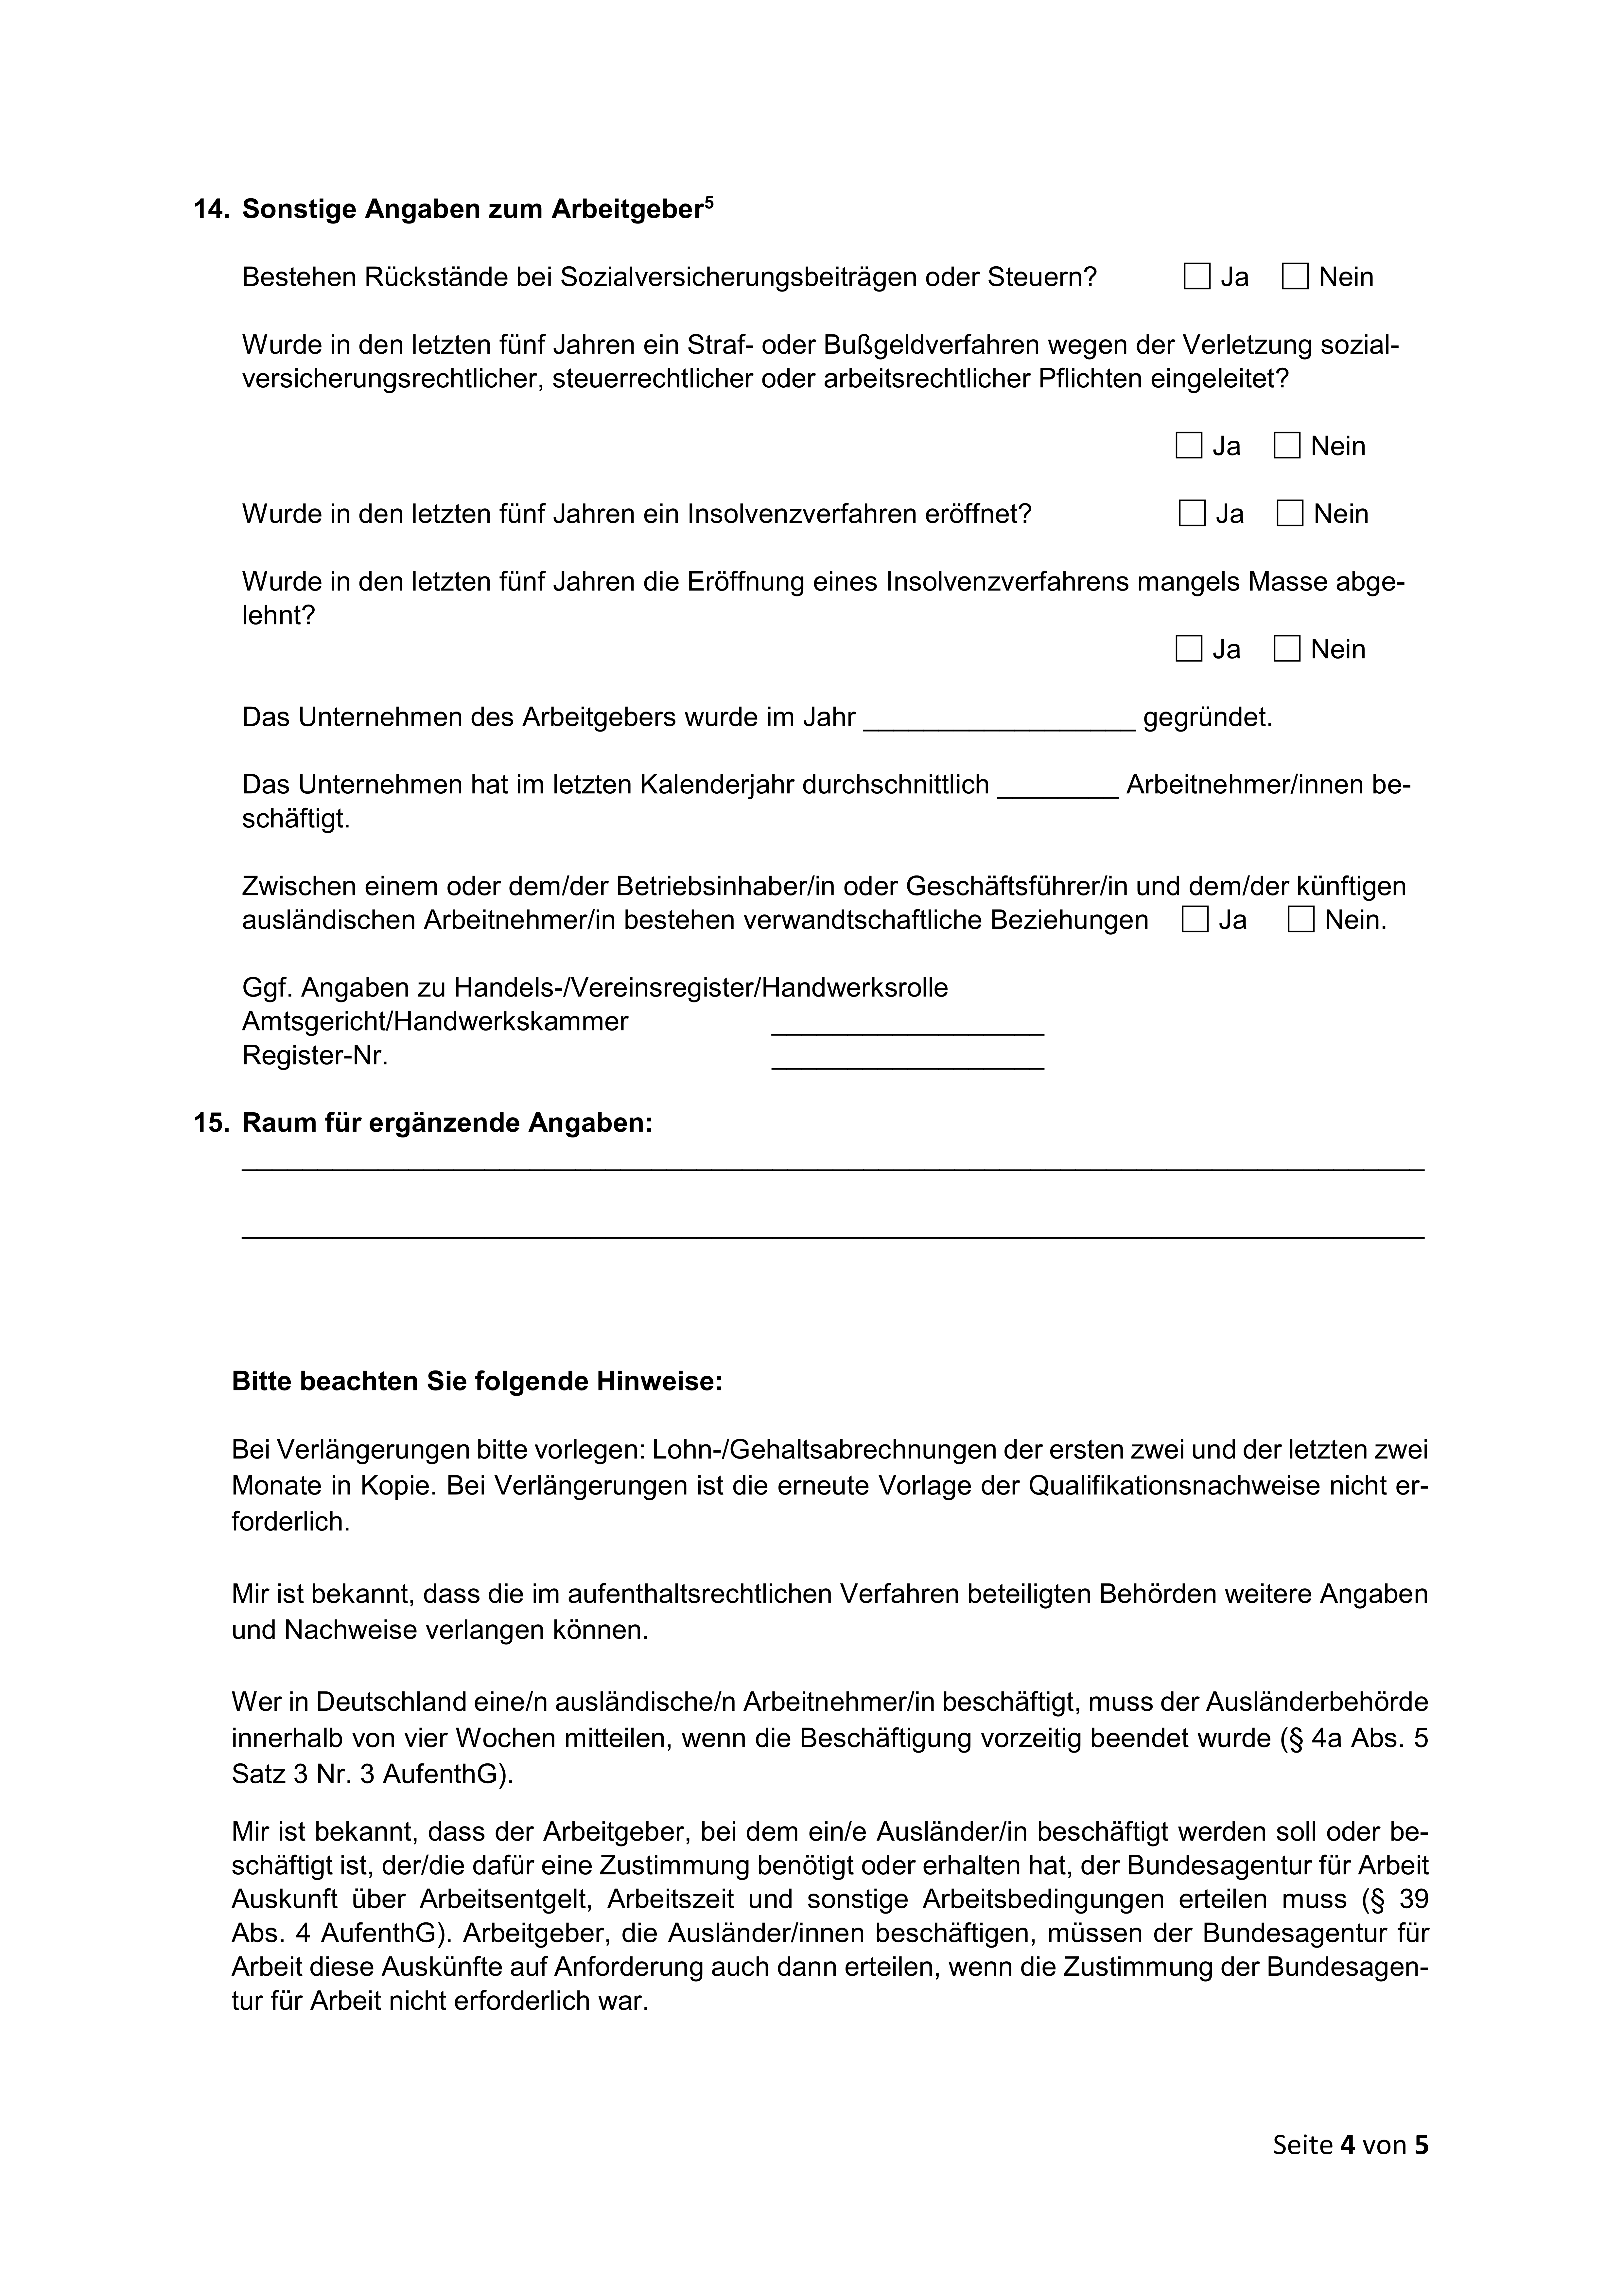
\includegraphics[width=\paperwidth,height=\paperheight]{s4_Erklaerung_zum_Beschaeftigungsverhaeltnis-000004}
  }%
}


 \BgThispage
%Berufsausübungserlaubnis
\begin{textblock*}{0.3cm\setstretch{1.75}}(15.4cm,3.489cm) % {block width} (coords)
\noindent
 \ifthenelse{\boolean{IsRueckstaendeSozSteu}}{x}{}
\end{textblock*}

\begin{textblock*}{0.3cm\setstretch{1.75}}(16.67cm,3.489cm) % {block width} (coords)
\noindent
 \ifthenelse{\boolean{IsRueckstaendeSozSteu}}{}{x}
\end{textblock*}

\begin{textblock*}{0.3cm\setstretch{1.75}}(15.3cm,5.7cm) % {block width} (coords)
\noindent
 \ifthenelse{\boolean{IsStrafBussgeld}}{x}{}
\end{textblock*}

\begin{textblock*}{0.3cm\setstretch{1.75}}(16.56cm,5.7cm) % {block width} (coords)
\noindent
 \ifthenelse{\boolean{IsStrafBussgeld}}{}{x}
\end{textblock*}

\begin{textblock*}{0.3cm\setstretch{1.75}}(15.34cm,6.56cm) % {block width} (coords)
\noindent
 \ifthenelse{\boolean{IsInsolvenz}}{x}{}
\end{textblock*}

\begin{textblock*}{0.3cm\setstretch{1.75}}(16.59cm,6.56cm) % {block width} (coords)
\noindent
 \ifthenelse{\boolean{IsInsolvenz}}{}{x}
\end{textblock*}

\begin{textblock*}{0.3cm\setstretch{1.75}}(15.32cm,8.35cm) % {block width} (coords)
\noindent
 \ifthenelse{\boolean{IsInsolvenzAbgelehnt}}{x}{}
\end{textblock*}

\begin{textblock*}{0.3cm\setstretch{1.75}}(16.58cm,8.35cm) % {block width} (coords)
\noindent
 \ifthenelse{\boolean{IsInsolvenzAbgelehnt}}{}{x}
\end{textblock*}

\begin{textblock*}{3.1cm\setstretch{1.75}}(11.2cm,9.2cm) % {block width} (coords)
\noindent
\Gruendungsjahr
\end{textblock*}

\begin{textblock*}{3.1cm\setstretch{1.75}}(12.9cm,10.05cm) % {block width} (coords)
\noindent
\AnzahlAN
\end{textblock*}

\begin{textblock*}{0.3cm\setstretch{1.75}}(15.37cm,11.83cm) % {block width} (coords)
\noindent
 \ifthenelse{\boolean{IsVerwandtschaft}}{x}{}
\end{textblock*}

\begin{textblock*}{0.3cm\setstretch{1.75}}(16.74cm,11.83cm) % {block width} (coords)
\noindent
 \ifthenelse{\boolean{IsVerwandtschaft}}{}{x}
\end{textblock*}

\begin{textblock*}{3cm\setstretch{1.75}}(10cm,13.12cm) % {block width} (coords)
\noindent
\Amtsgericht
\end{textblock*}

\begin{textblock*}{3cm\setstretch{1.75}}(10cm,13.57cm) % {block width} (coords)
\noindent
\Registernummer
\end{textblock*}

\begin{textblock*}{15.4cm\setstretch{2.05}}(3.16cm,14.87cm) % {block width} (coords)
\noindent
\WeitereAngabenSvier
\end{textblock*}

~\clearpage

\backgroundsetup{
scale=1,
color=black,
opacity=1,
angle=0,
contents={%
  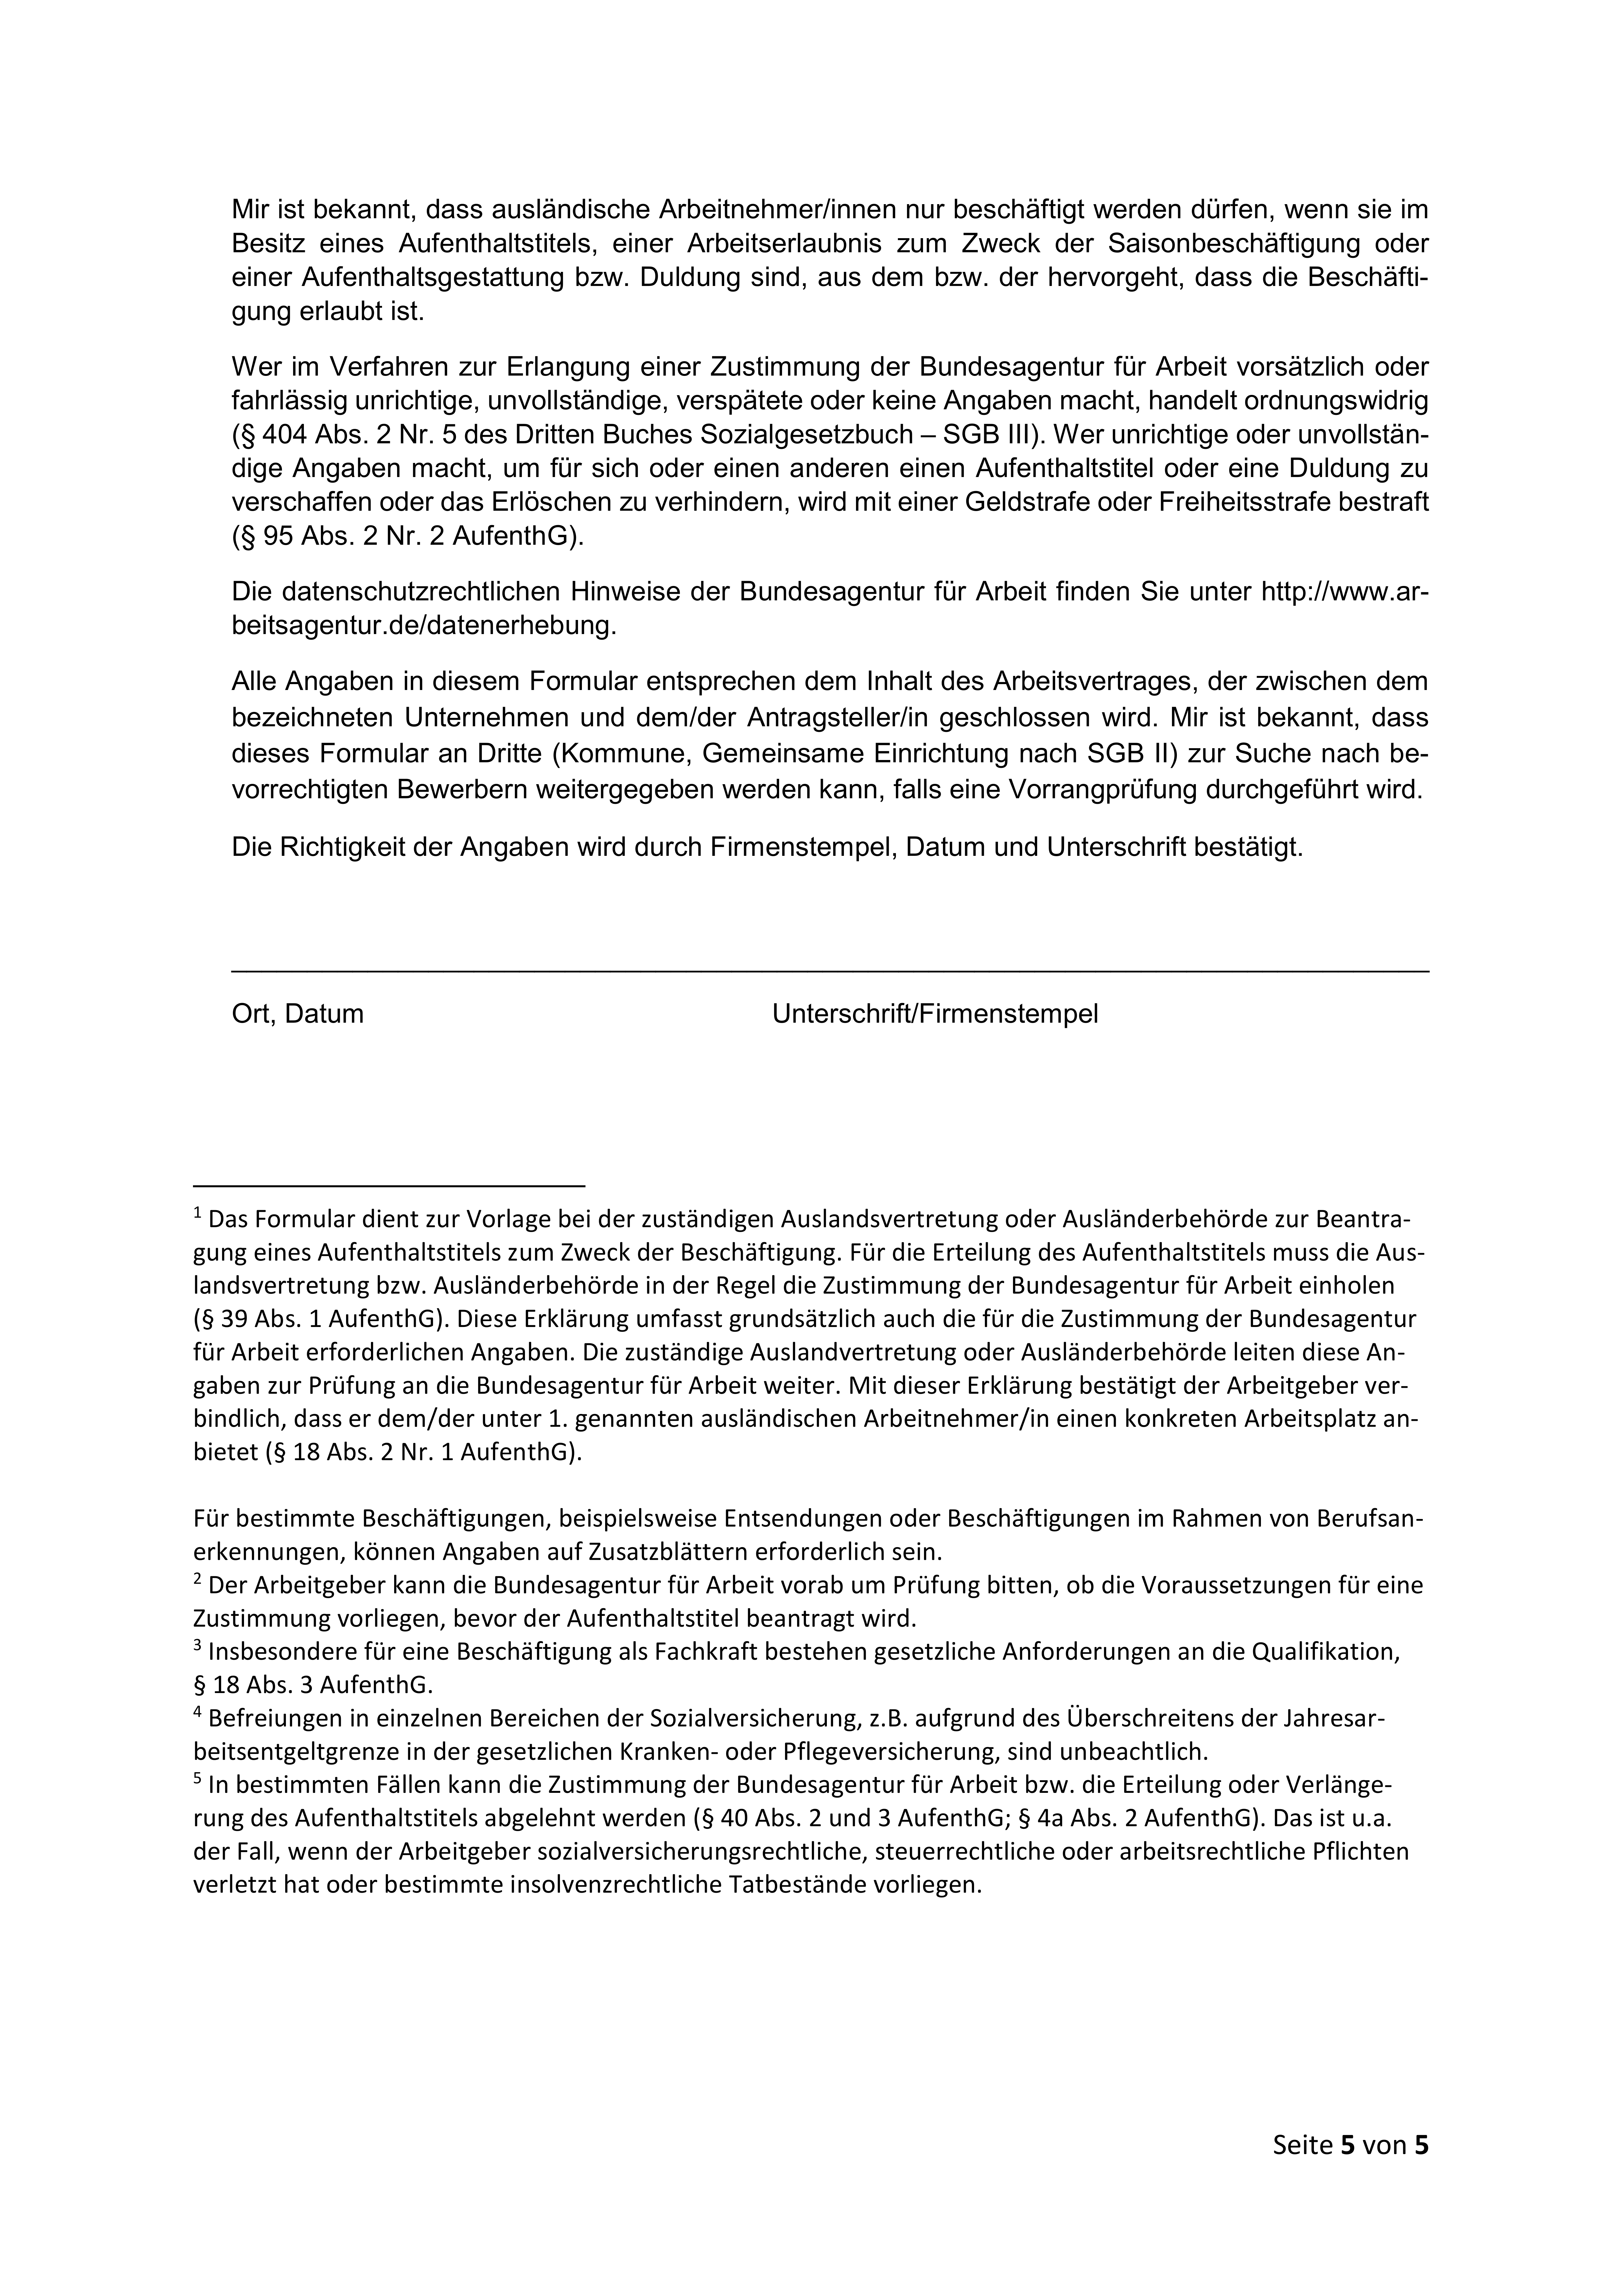
\includegraphics[width=\paperwidth,height=\paperheight]{s5_Erklaerung_zum_Beschaeftigungsverhaeltnis-000005}
  }%
}
\BgThispage

%Text
\begin{textblock*}{7cm\setstretch{1.75}}(3cm,12.3cm) % {block width} (coords)
\noindent
\OrtDatum
\end{textblock*}

\clearpage
\end{Form}
\end{document}
